\documentclass[10pt]{article}
\usepackage[utf8]{inputenc}
\usepackage[T1]{fontenc}
\usepackage{graphicx}
\usepackage[export]{adjustbox}
\graphicspath{ {./images/} }
\usepackage{amsmath}
\usepackage{amsfonts}
\usepackage{amssymb}
\usepackage[version=4]{mhchem}
\usepackage{stmaryrd}
\usepackage{caption}

\title{Microgrids }

\author{}
\date{}


\begin{document}
\maketitle
\captionsetup{singlelinecheck=false}
ELEN0445\\
Operational planning

Introduction\\
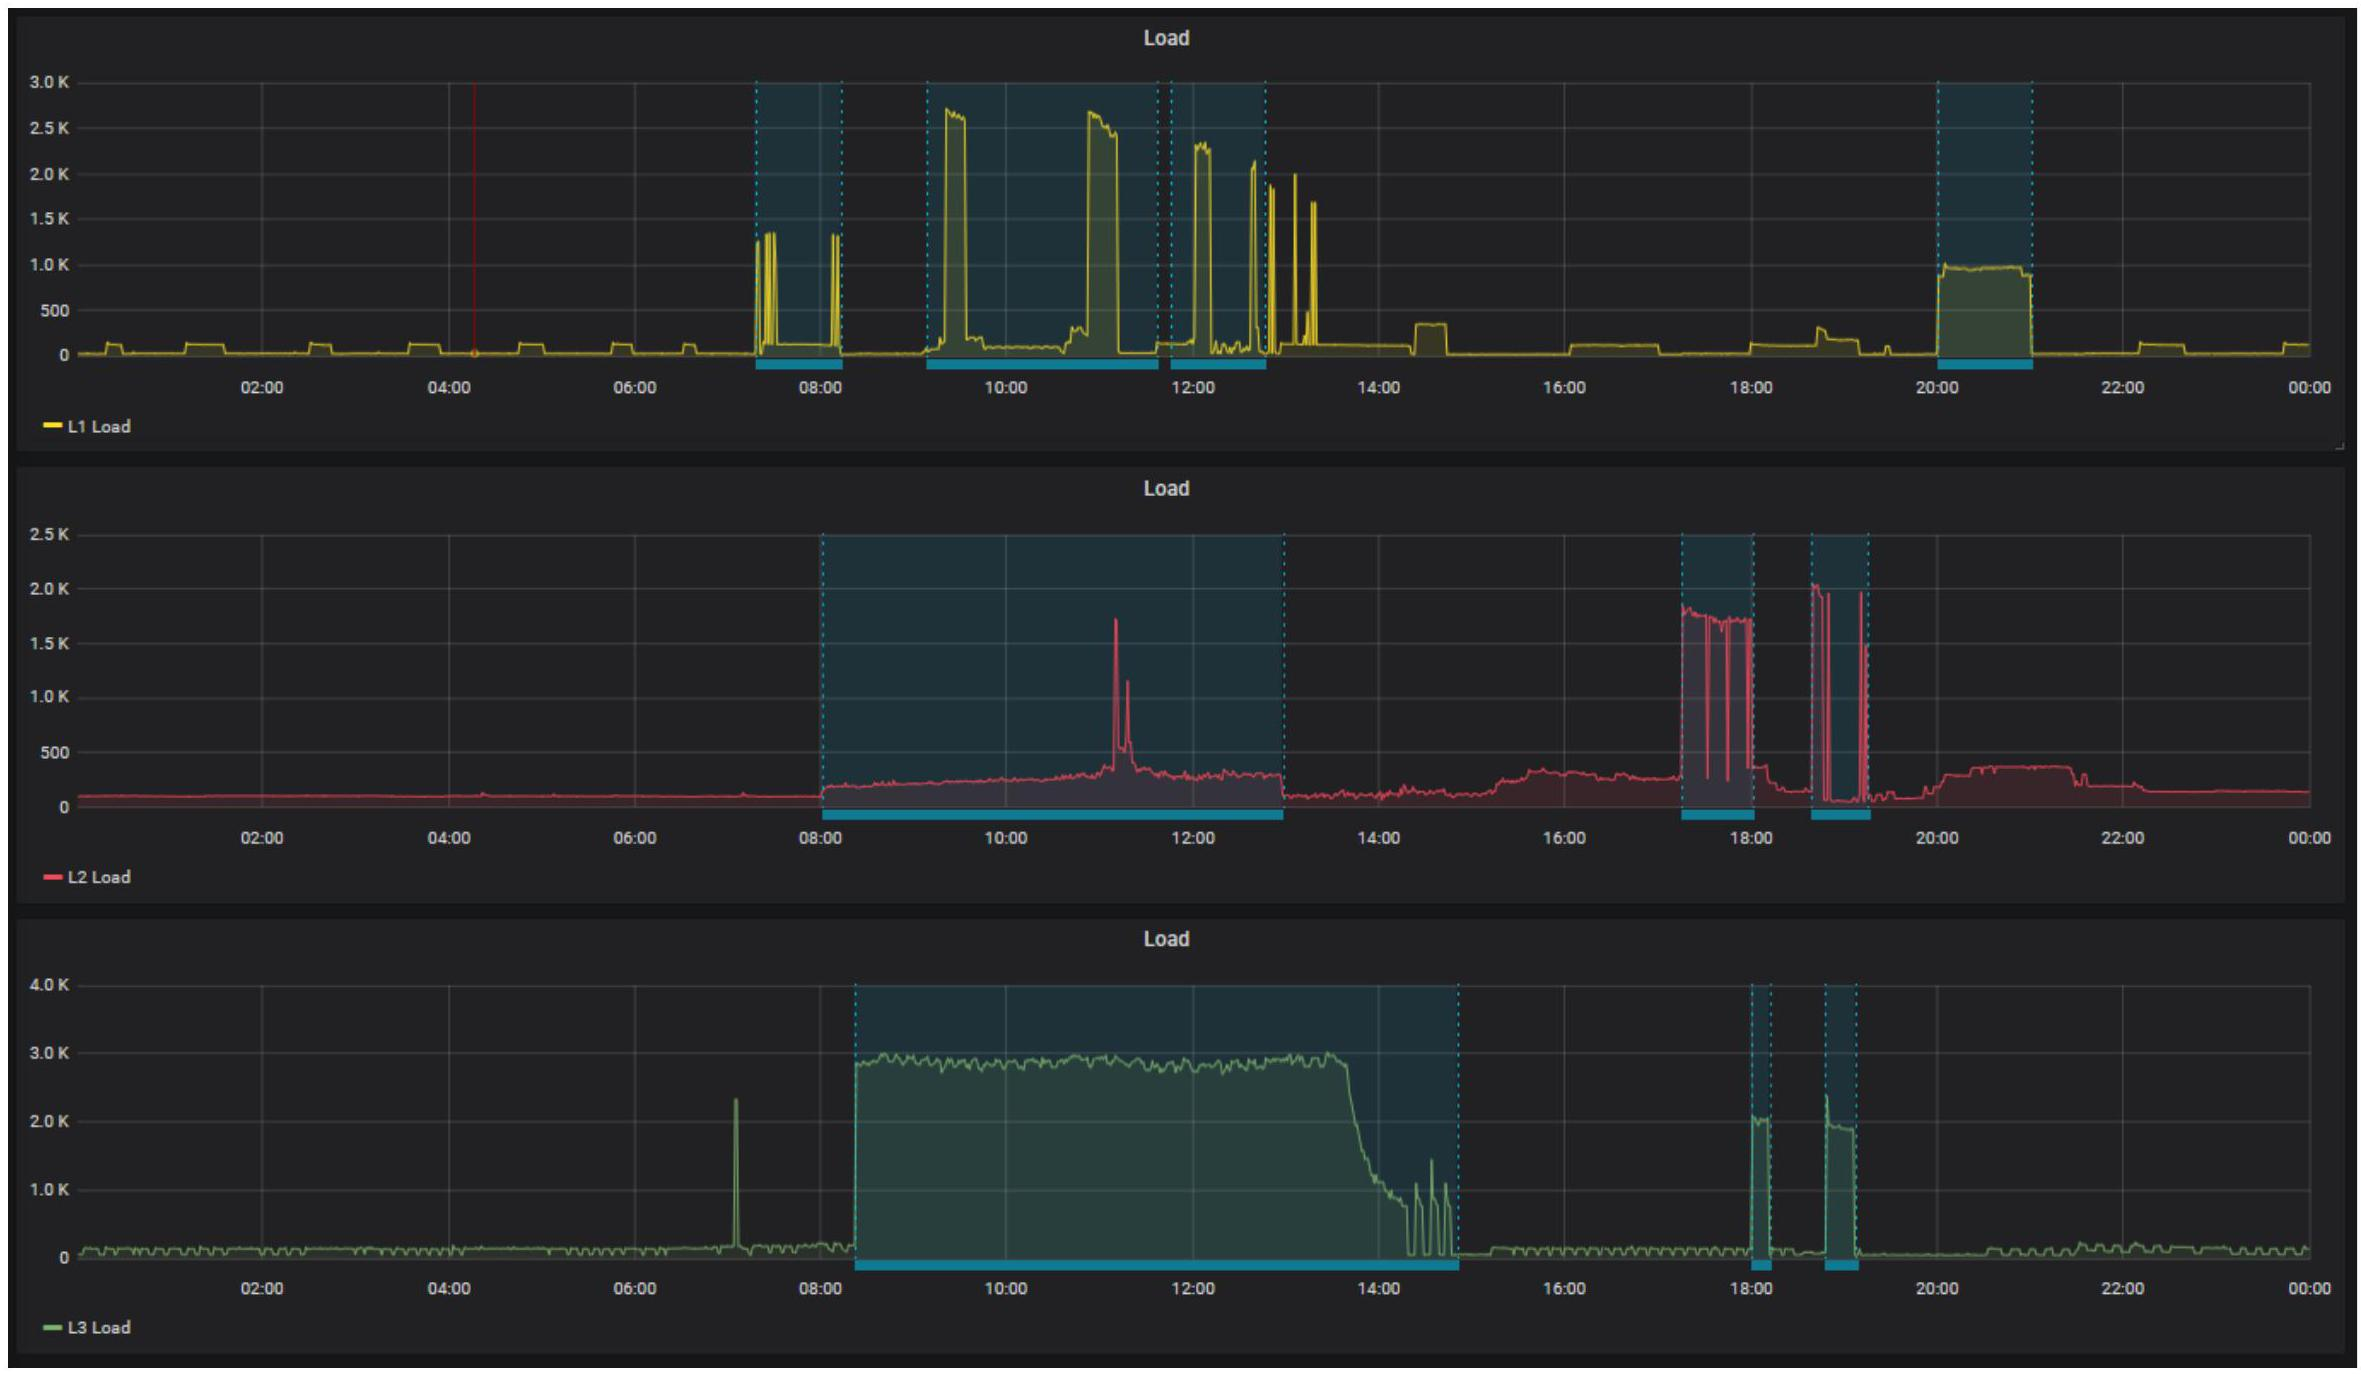
\includegraphics[max width=\textwidth, alt={}, center]{4f5abcf0-f301-43b5-aaf0-9e34a9c79ca8-03_1374_2361_286_484}\\
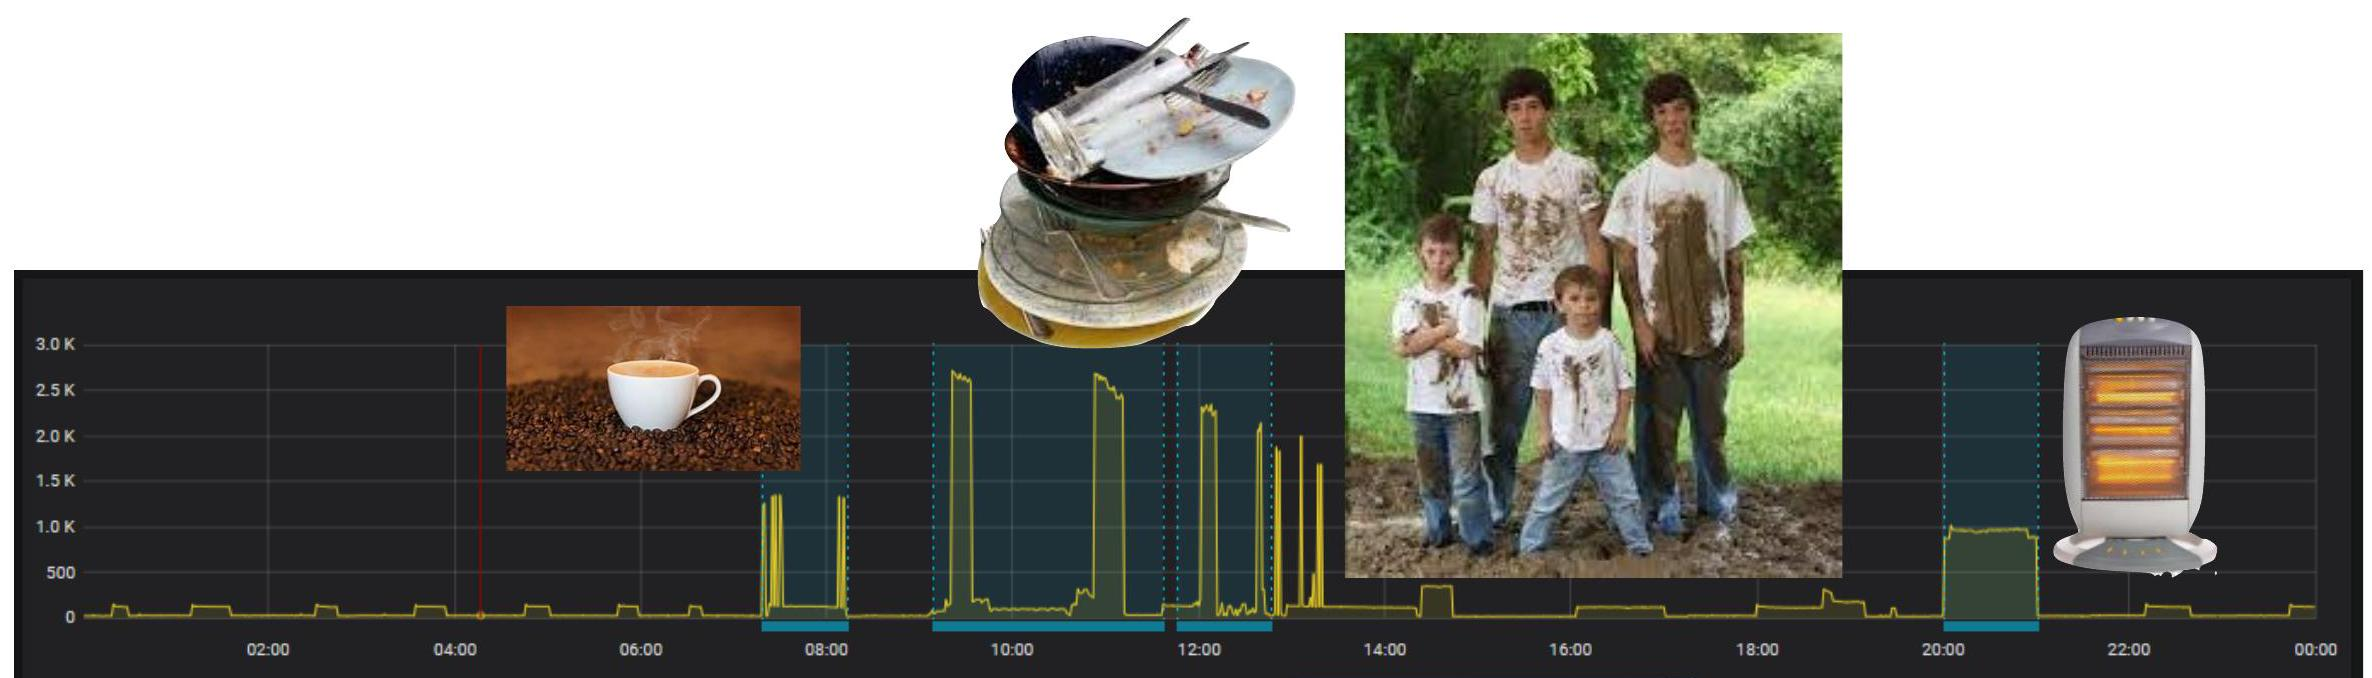
\includegraphics[max width=\textwidth, alt={}, center]{4f5abcf0-f301-43b5-aaf0-9e34a9c79ca8-04_678_2372_24_478}\\
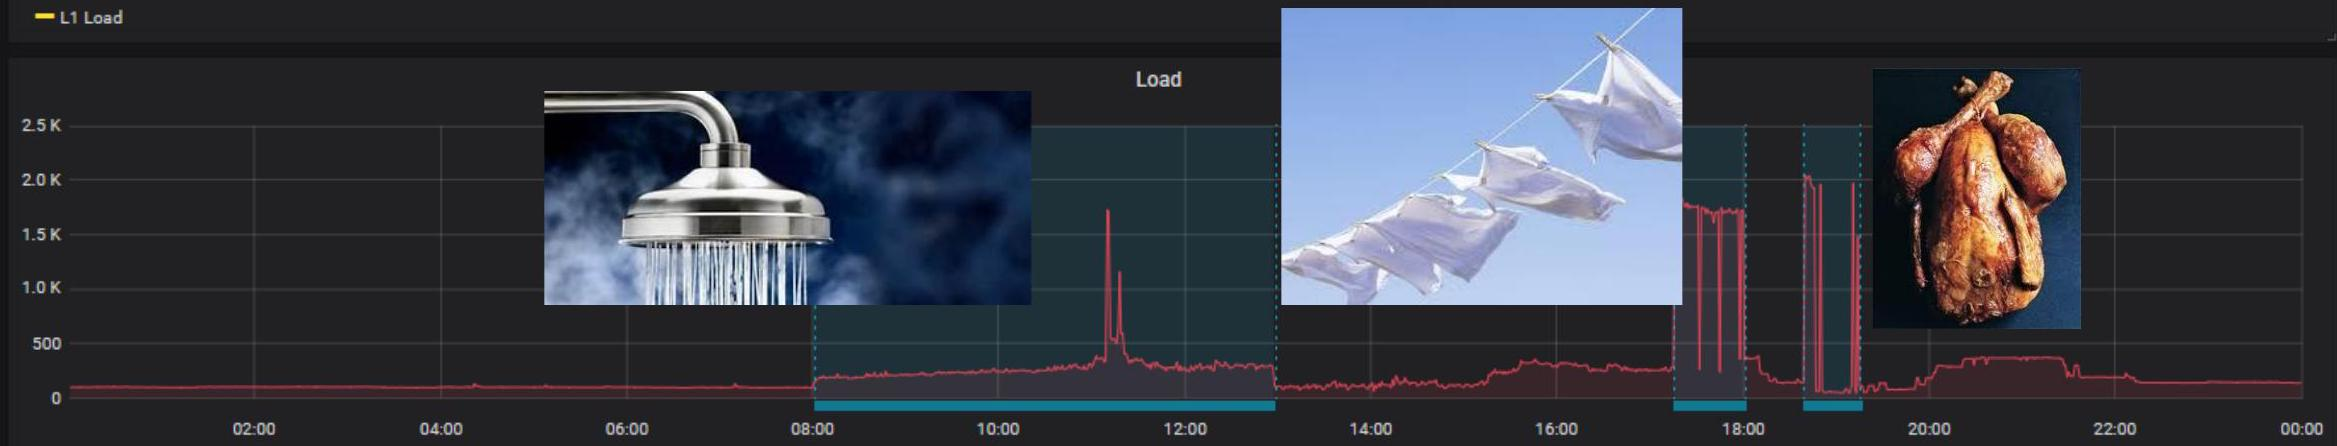
\includegraphics[max width=\textwidth, alt={}, center]{4f5abcf0-f301-43b5-aaf0-9e34a9c79ca8-04_446_2337_695_492}

\begin{itemize}
  \item L2 Load\\
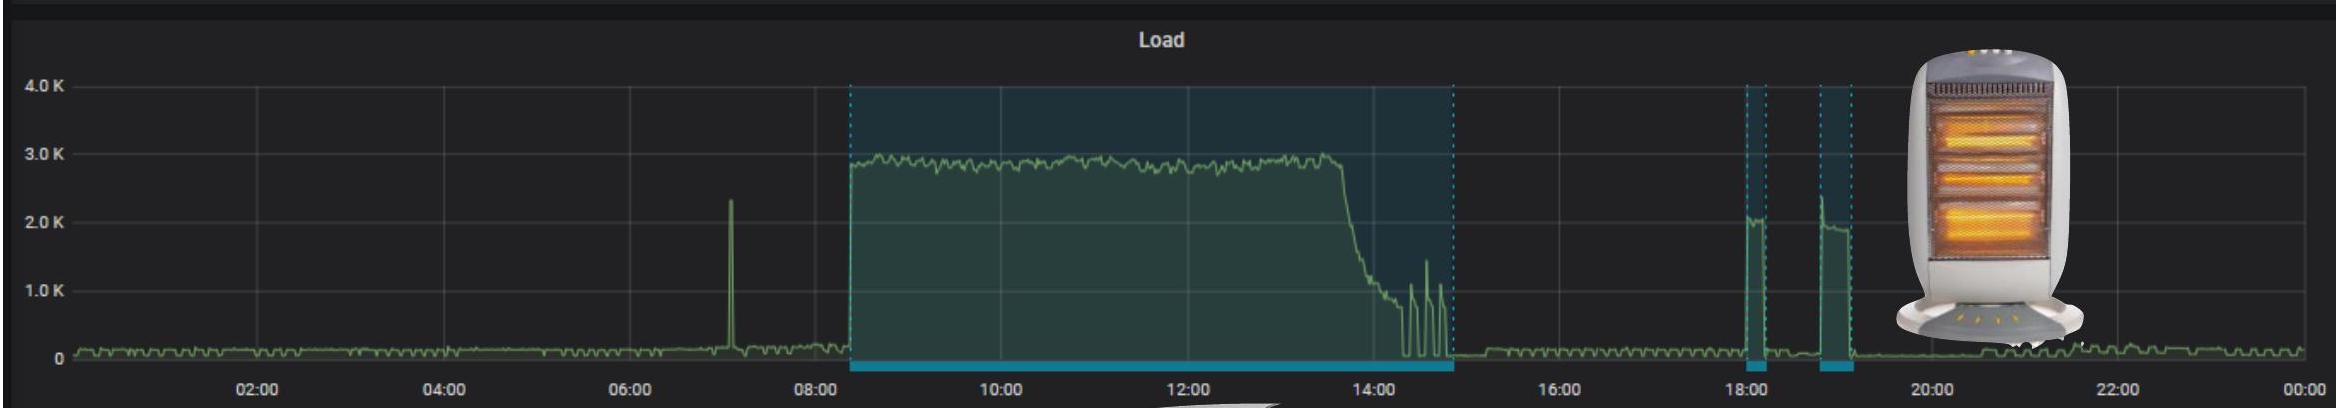
\includegraphics[max width=\textwidth, alt={}, center]{4f5abcf0-f301-43b5-aaf0-9e34a9c79ca8-04_408_2336_1185_489}\\

\includegraphics[max width=\textwidth, alt={}, center]{4f5abcf0-f301-43b5-aaf0-9e34a9c79ca8-04_32_111_1599_515}
\end{itemize}

LIÈGE université\\
Sciences Appliquées\\
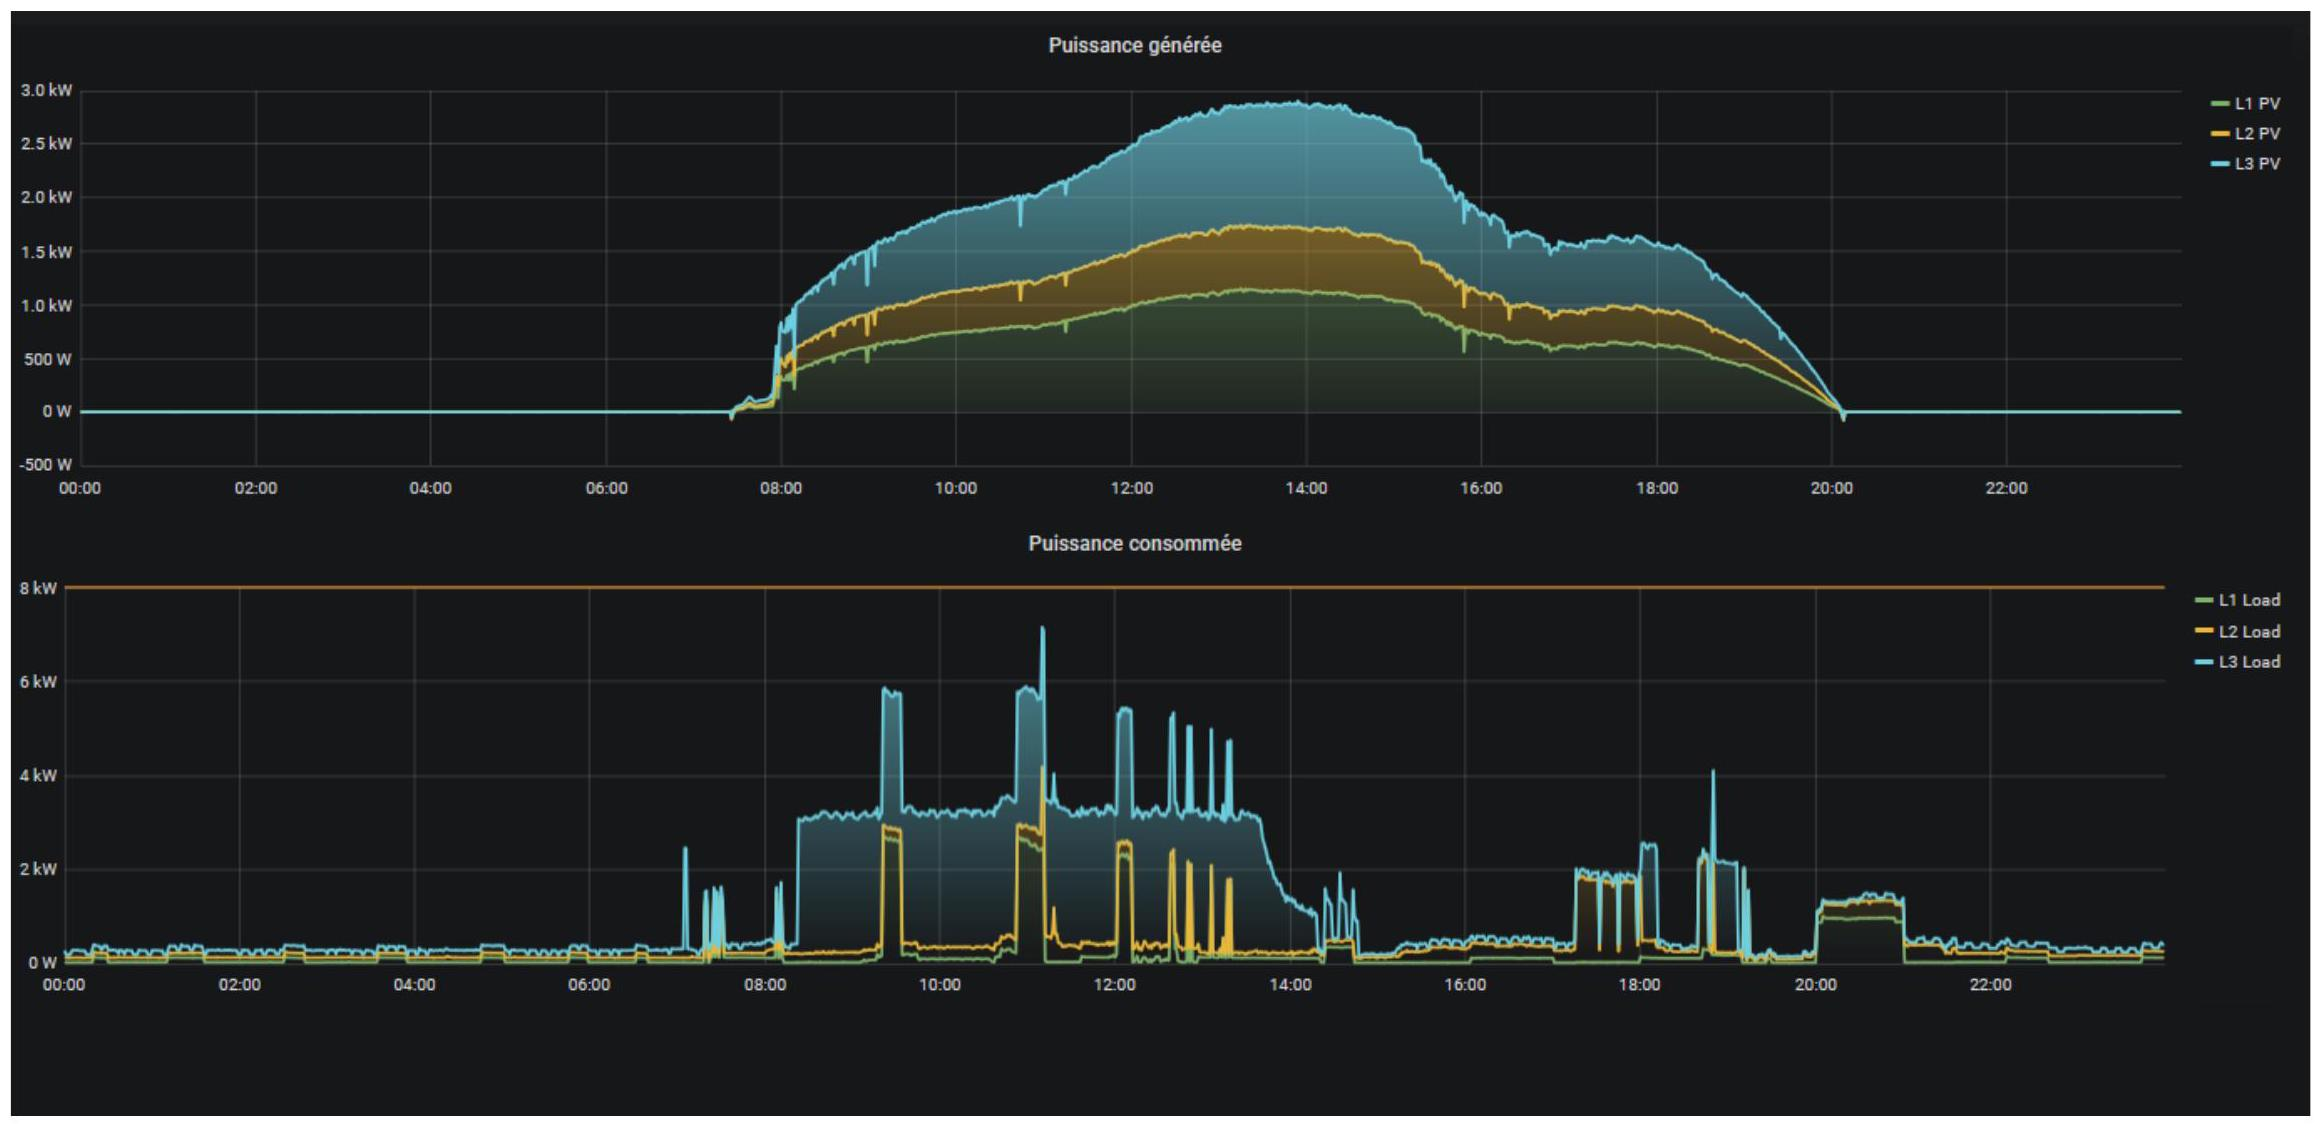
\includegraphics[max width=\textwidth, alt={}, center]{4f5abcf0-f301-43b5-aaf0-9e34a9c79ca8-05_1124_2317_429_510}

\section*{Content of this lecture}
\begin{itemize}
  \item We take the role of the operator of the microgrid, who wants to optimize the way the energy is produced and used within the microgrid, and to optimize the interaction with the public grid (simple interaction, e.g. varying price).
  \item We make the assumptions that the microgrid is single-user, and we also avoid the question of the "fast dynamics" of the components of the microgrid.
\end{itemize}

\section*{Reminder: control levels}
\begin{center}
\begin{tabular}{|l|l|l|}
\hline
Level & Function & Examples \\
\hline
1 & Device level control & BSS control, reactive control \\
\hline
2 & Local area control & Frequency regulation, fast load shedding \\
\hline
3 & Supervisory control & Forecasting, operational planning \\
\hline
4 & Public Grid interaction & Ancillary services, energy markets \\
\hline
\end{tabular}
\end{center}

We will be mainly focused on levels 3 and 4, and a bit about level 2

In this lecture: level 3 \& centralized control

Operational planning

\section*{When are operation decisions taken?}
\begin{itemize}
  \item It can be in real time: corrective decisions
  \item Or in anticipation: preventive decisions
  \item Why should we anticipate? because of time coupling constraints:
  \item The typical periodicity of renewable generation devices and consumption is a day
  \item Human activity has daily, weekly and seasonal periodicity
\end{itemize}

\section*{Operational planning decision horizon T}
\begin{itemize}
  \item We cannot take preventive operation decisions too much in advance:
  \item too high uncertainty on the evolution of the state of the microgrid and its environment
  \item anticipating a bit on the sequel, the problem we will have to solve may be intractable
  \item We thus consider operating the system over one day to approx. one week. This can be more or less, depending on the particular situation of the microgrid (type of storage, type of business activity, etc.)\\
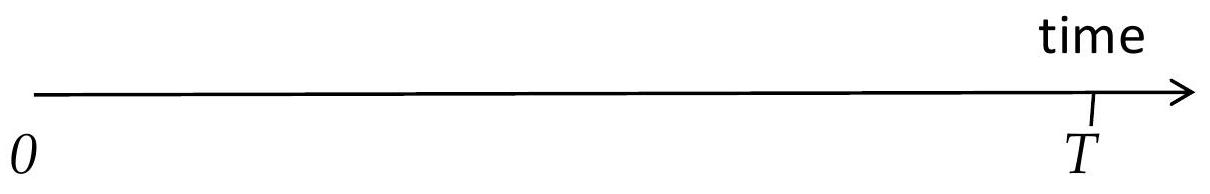
\includegraphics[max width=\textwidth, alt={}, center]{4f5abcf0-f301-43b5-aaf0-9e34a9c79ca8-11_194_1210_1495_1043}
\end{itemize}

\section*{Operational planning decision duration $\Delta_{t}$}
\begin{itemize}
  \item For computational reasons, we discretize the decisions in time
  \item Depending on the decision horizon, we may consider periods of 1 to 15 minutes where decisions are assumed constant
  \item Example: constant charge power for a battery
  \item Determining good decisions may become intractable if we have too many decisions in the decision horizon
  \item Forecasts may anyway not be meaningful with a too high temporal resolution
  \item This is coherent with market period duration\\
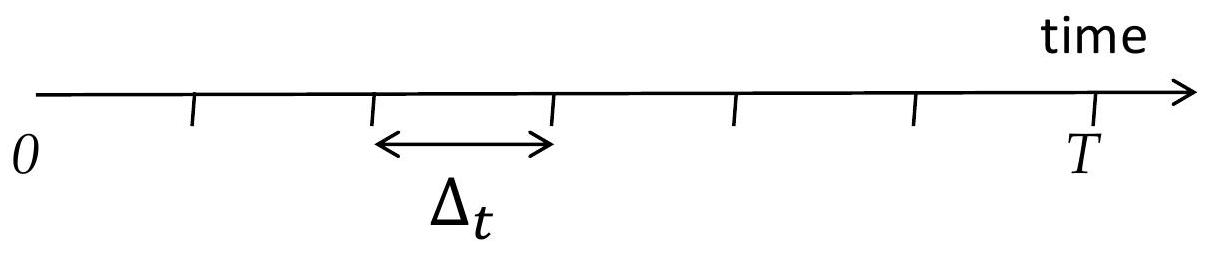
\includegraphics[max width=\textwidth, alt={}, center]{4f5abcf0-f301-43b5-aaf0-9e34a9c79ca8-12_257_1207_1495_1041}
\end{itemize}

\section*{Operation as a sequential decision-making problem}
We have a discrete-time system represented by a state $x_{t}$\\
$x=\left(x_{0}, x_{1}, \ldots, x_{T}\right)$ represents the state evolution of the system\\
$u=\left(u_{0}, \ldots, u\right.$ T-1 $)$ is a sequence of control actions (decisions)\\
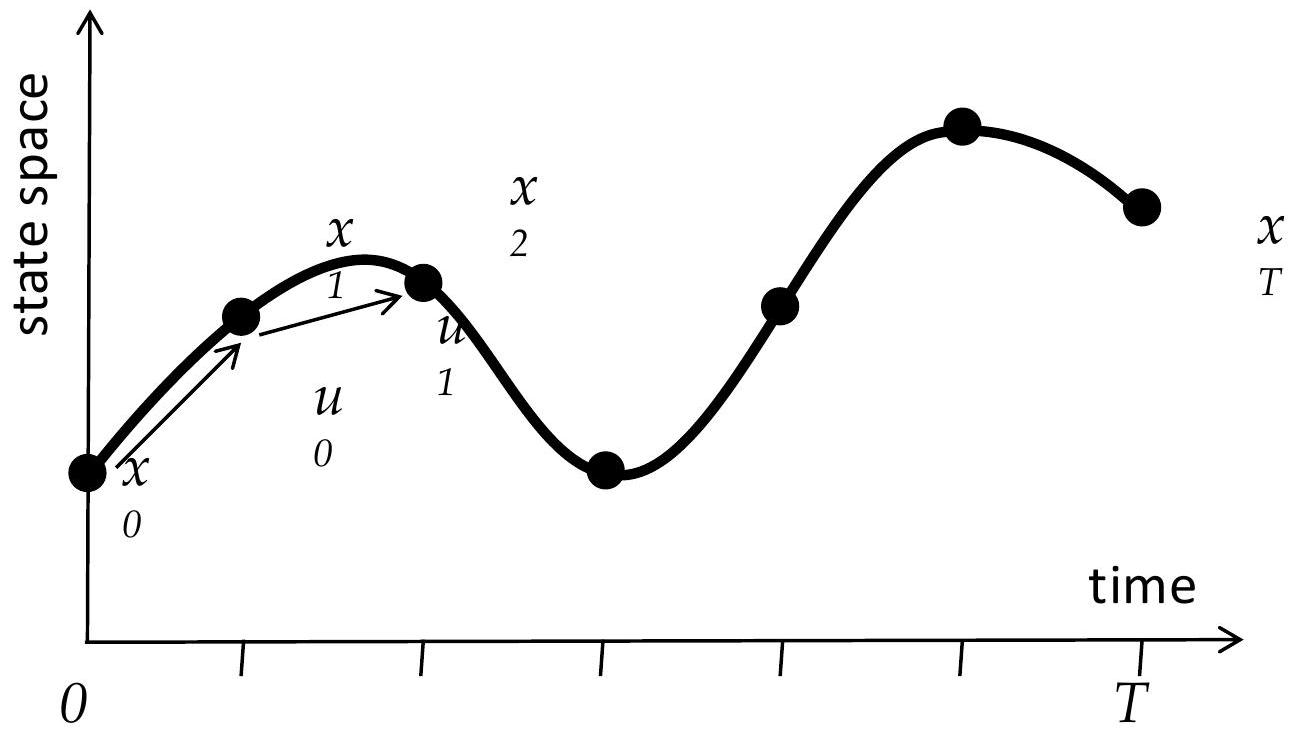
\includegraphics[max width=\textwidth, alt={}, center]{4f5abcf0-f301-43b5-aaf0-9e34a9c79ca8-13_736_1295_945_992}

\section*{Given a criterion, we can compute an openloop sequence of actions $\boldsymbol{u}^{*}$ to drive the system }
We estimate demand, generation, availability of system components, etc. and then solve\\
minimize cost of $u$\\
subject to 1 . balance generation and demand $\forall t \in\{1,2, \ldots, T\}$\\
2. dynamics: $x_{t-1}, u_{t-1} \rightarrow x_{t} \forall t \in\{1,2, \ldots, T\}$\\
3. action sequence and state evolution restrictions\\
4. initial state $x_{0}$

\section*{Uncertainty}
\begin{itemize}
  \item Microgrid operation is impacted by factors that are not easily predictable
  \item the weather, which impacts renewable generation and consumption
  \item outages of steerable generation or storage
  \item Some events may thus turn the open-loop sequence $u^{*}$ suboptimal or infeasible
  \item This can be mitigated by the a receding horizon approach
\end{itemize}

\section*{Receding horizon approach}
Example: demand variation or restriction on $x$ or $u$ are observed at time $t_{r}$\\
Receding horizon approach: update the sequence of control actions

\begin{enumerate}
  \item Re-estimate the parameters (demand, availabilities)
  \item Re-solve the open-loop formulation\\
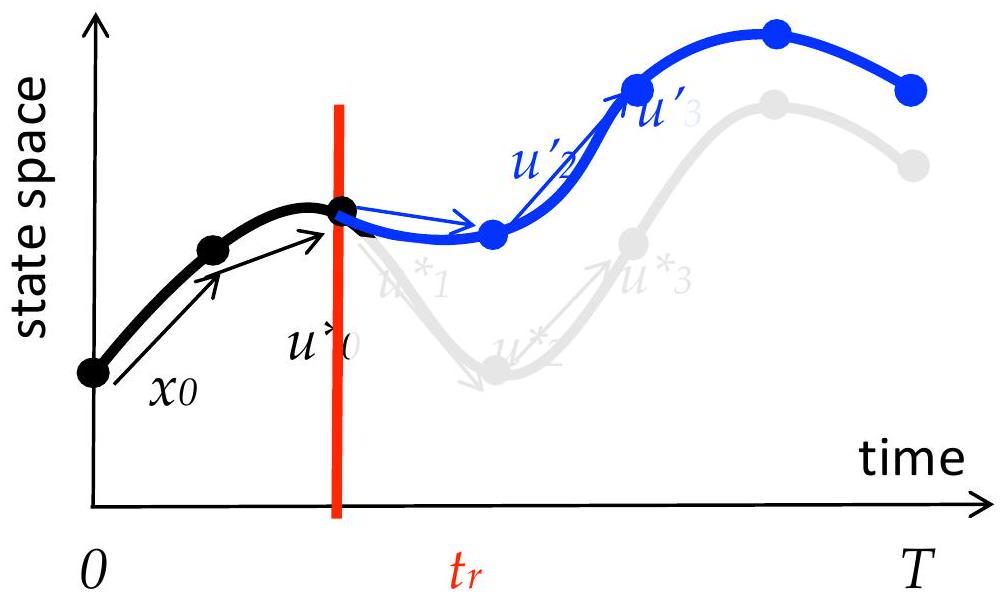
\includegraphics[max width=\textwidth, alt={}, center]{4f5abcf0-f301-43b5-aaf0-9e34a9c79ca8-16_603_1007_1010_1067}\\
$x_{T}$
\end{enumerate}

\section*{So, finally, when are decisions applied?}
\begin{itemize}
  \item Every time we solve the optimization problem above, we "freeze" some decisions:
  \item not only the decisions occurring before the next reoptimization
  \item but also decisions that have a high impact on the interactions within the microgrid or with the public grid, and that span the whole decision horizon
  \item Hence, depending on the moment of the day, some decisions may or not be re-optimized
\end{itemize}

\section*{Decisions, in practice}
\begin{itemize}
  \item Storage devices: Set point for charging / discharging
  \item Steerable generation
  \item Non-steerable renewable generation: curtailment
  \item Load shedding
  \item Load flexibility\\
-Power electronics
\end{itemize}

\section*{Remark: decisions we do not consider}
We do not consider investment decisions

\begin{itemize}
  \item This is the topic of another topic on sizing
\end{itemize}

We do not consider maintenance decisions

\begin{itemize}
  \item Maintenance cost can be accounted for in sizing
  \item In operation, scheduled maintenance are just extra constraints or data updates (e.g. PV is out)
  \item If necessary, maintenance scheduling could be stated as an extension of operational planning
\end{itemize}

\section*{Constraints, in practice}
\begin{itemize}
  \item Capacity of devices
  \item Inverters constraints
  \item Demand-side management
  \item Generation management
  \item Regularization:
  \item avoid changing decisions if unnecessary/undesirable
\end{itemize}

Optimization objectives

\section*{The invoice}
\begin{itemize}
  \item (In Belgium), the invoice of a user connected to a distribution network is composed of:
  \item A part proportional to the energy consumed
  \item A part proportional to the capacity of the connection, i.e. the amount of power the user can withdraw from the distribution grid
  \item A part proportional to the "cos phi"
  \item Taxes and other contributions
  \item This varies a lot as a function of the type of connection (i.e. of the voltage level and overall consumption)
\end{itemize}

\section*{Minimize the energy purchase cost}
\begin{itemize}
  \item The microgrid is subject to a dynamic price signal. At every time $t$, it can buy electricity at a price $p_{t}$
  \item Then, it will try to
  \item consume $\&$ charge the storage devices during low price periods
  \item produce \& discharge the storage devices during high price periods
  \item Note: for now, we consider that
  \item the microgrid cannot influence the price
  \item there is no imbalance penalty
  \item on the other hand, we will not always assume the price is known in advance.
\end{itemize}

\section*{Maximize the electricity sale price}
\begin{itemize}
  \item In a similar way, the price at which a retailer will buy back the energy can be described as a vector of prices, one per hour of the day.
  \item At a time $t$, the sale price is obviously always lower than the purchase price:
  \item because the retailer takes a margin
  \item because the purchase price includes the grid fees, taxes, etc.
  \item There may be an injection fee depending on the DSO
\end{itemize}

\section*{Minimize the peak}
\begin{itemize}
  \item A grid user pays a monthly fee function of his peak quarter-hourly consumption over the last 12 months.
  \item Remark: this introduces a huge time coupling in the operation problem.
\end{itemize}

\section*{Maximize the reserve}
\begin{itemize}
  \item Keeping some reserve, i.e. some flexibility to quickly change the net position (total generation - total consumption) of the microgrid is important for two reasons:
  \item It can be used to sell ancillary services to the grid
  \item It can be used to stabilize the microgrid, in islanded mode.
\end{itemize}

\section*{In summary}
\begin{itemize}
  \item Costs
\end{itemize}

\begin{itemize}
  \item Energy consumption
  \item Peak penalty
\end{itemize}

\begin{itemize}
  \item Revenues\\
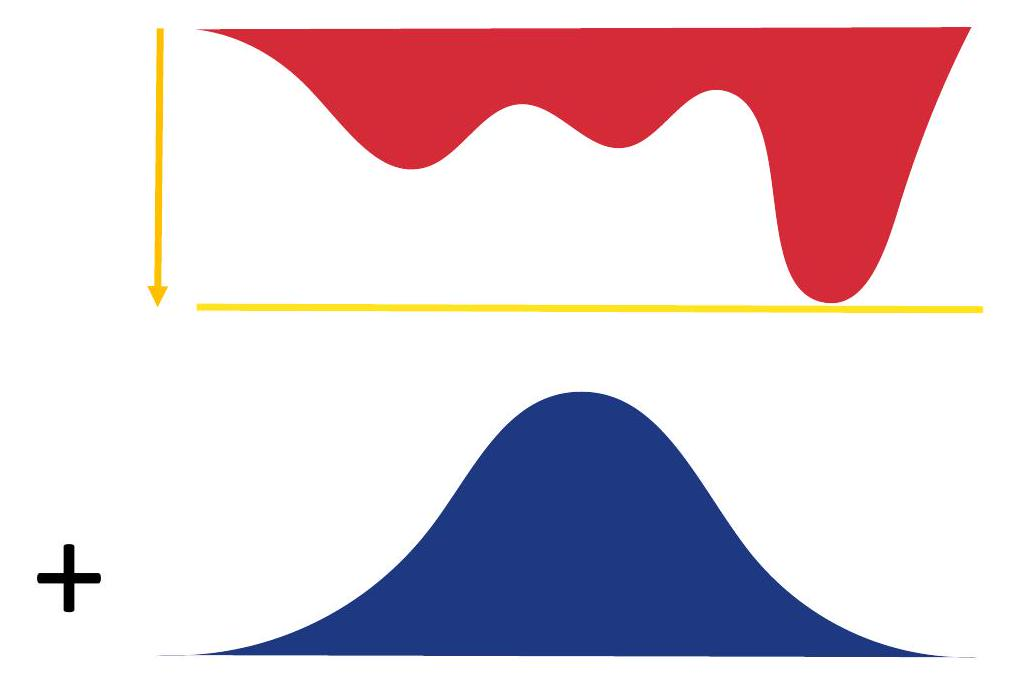
\includegraphics[max width=\textwidth, alt={}, center]{4f5abcf0-f301-43b5-aaf0-9e34a9c79ca8-27_681_1009_452_1414}
\end{itemize}

\begin{itemize}
  \item Energy production
\end{itemize}

\begin{itemize}
  \item Ancillary services\\
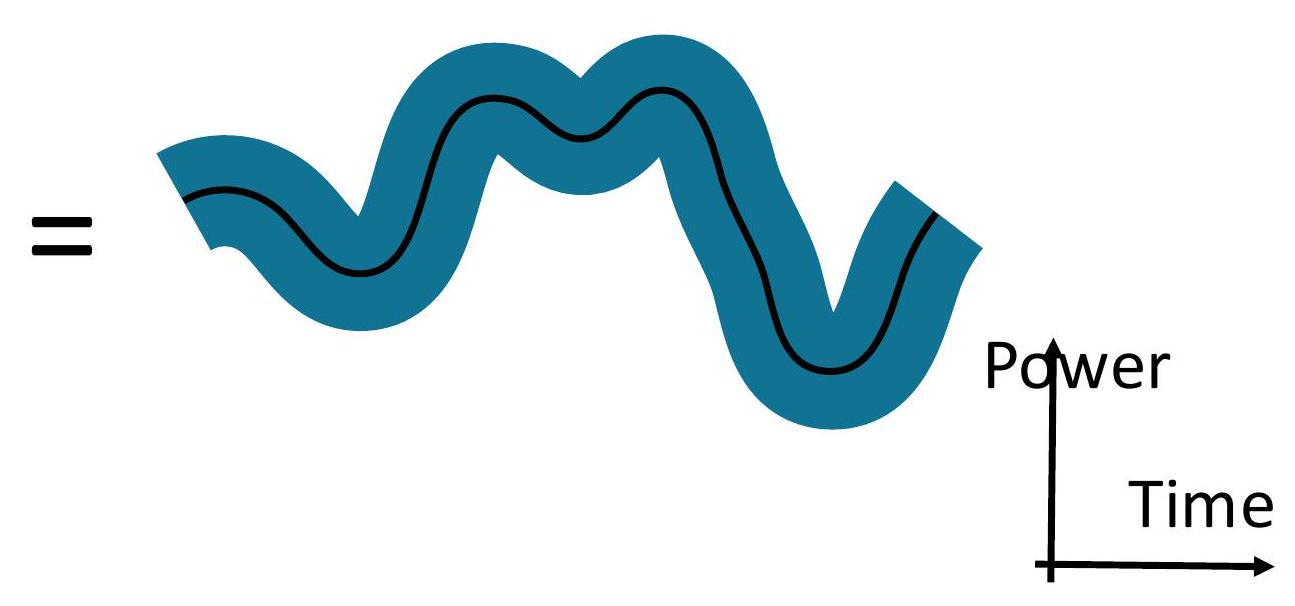
\includegraphics[max width=\textwidth, alt={}, center]{4f5abcf0-f301-43b5-aaf0-9e34a9c79ca8-27_606_1295_1195_1414}
\end{itemize}

\section*{Minimize components' degradation}
\begin{itemize}
  \item Generation devices, such as internal combustion machines, have a lifetime which varies significantly with the way they are used.
  \item Batteries suffer of the same problem. However, this depends a lot with the type of battery technology.
\end{itemize}

\section*{(Islanded mode) Ensure security of supply}
In case of public grid service interruption, the objective of the microgrid may suddenly switch to simply keeping the critical loads powered as long as possible.

\section*{All these objectives are (most of the time) conflictual}
\begin{itemize}
  \item For instance:
  \item Minimizing the peak can lead to opportunity losses with respect to low energy purchase prices
  \item Maintaining a level of reserve can lead to peak increases and also to some opportunity losses with respect to energy purchase/sale price
  \item Minimizing component degradation should be put in perspective with the opportunity losses it generates
  \item Hence we must reach a tradeoff between these objectives
\end{itemize}

Load models for demand-side management

\section*{What are the electrical devices in your house?}
On the demand side

\begin{itemize}
  \item Lights
  \item Fridges
  \item TV, computer, etc.
  \item Dishwasher
  \item Washing machine
  \item Tumble dryer
  \item Electrical vehicle
  \item Hot water boiler
  \item Heat pump
  \item Direct heating
  \item Pumps
  \item etc.
\end{itemize}

\section*{How can you characterize these loads?}
\begin{itemize}
  \item Power rating (kW, kVA, kvar)
  \item Power consumption pattern
  \item Energy consumption
  \item Efficiency
  \item Flexibility
  \item Controllability
  \item Behavior w.r.t. voltage variation, frequency variation
\end{itemize}

\section*{The next models are inspired from}
\begin{itemize}
  \item Roh, H. T., \& Lee, J. W. (2015). Residential demand response scheduling with multiclass appliances in the smart grid. IEEE Transactions on Smart Grid, 7(1), 94-104.
\end{itemize}

\section*{Loads can be subdivided in 5 categories}
\begin{itemize}
  \item Elastic / Inelastic
  \item MemoryLess, with Full Memory or Partial Memory
  \item Interruptible or UnInterruptible
\end{itemize}

\begin{center}
\begin{tabular}{|c|l}
\hline
Set &  \\
\hline
$\boldsymbol{A}_{E M L}$ & light bulbs with controllable brightness, electric fans with controllable speeds \\
\hline
$\boldsymbol{A}_{E F M}$ & battery chargers (electric vehicles) with controllable charging rates \\
\hline
$\boldsymbol{A}_{E P M}$ & electric heaters, air conditioners, refrigerators \\
\hline
$\boldsymbol{A}_{I E I}$ & battery chargers (electric vehicles) with fixed charging rates, computers with in \\
\hline
$\boldsymbol{A}_{I E U I}$ & washing machines, dishwashers, electric ovens, televisions, light bulbs without \\
\hline
\end{tabular}
\end{center}

\section*{A model is proposed for each category}
\begin{itemize}
  \item Let $x_{a}^{t}$ be the consumption of appliance $a$ at time $t$
  \item Let $y_{a}^{t}$ be an integer variable that denotes whether appliance $a$ starts at time $t$
  \item Parameters define limits on $x_{a}^{t}\left(x_{a}^{m i n}, x_{a}^{m a x}\right)$, minimum performance thresholds of appliances' performance ( $R_{a}, R_{a}^{t}$ ), energy consumption for inelastic ones ( $E_{a}$ ), etc.
\end{itemize}

\section*{E.g. elastic with full memory loads (EFM)}
Each appliance $a$ also has the maximum and minimum values for its energy consumption, $x_{a}^{\max }$ and $x_{a}^{\min }$, respectively, at each sub-interval $t$, that is


\begin{equation*}
x_{a}^{\min } \leq x_{a}^{t} \leq x_{a}^{\max }, \quad \forall t \in \boldsymbol{T}_{a}, \forall a \in \boldsymbol{A}_{\mathrm{EFM}} . \tag{10}
\end{equation*}


Each appliance $a$ has its utility function $U_{a}\left(\boldsymbol{x}_{a}\right)$, which is defined as


\begin{equation*}
U_{a}\left(\boldsymbol{x}_{a}\right)=U_{a}\left(\sum_{t \in \boldsymbol{T}_{a}} x_{a}^{t}\right), \quad \forall a \in \boldsymbol{A}_{\mathrm{EFM}} . \tag{11}
\end{equation*}


\section*{(...)}
We also assume that the utility function is a concave function. In addition, we assume that for each appliance $a$, its user has the following requirement:


\begin{equation*}
U_{a}\left(\boldsymbol{x}_{a}\right) \geq R_{a}, \quad \forall a \in \boldsymbol{A}_{\mathrm{EFM}} \tag{12}
\end{equation*}


This requirement indicates that the performance of appliance $a$ that depends on its total energy consumption should be higher than or equal to its minimum threshold $R_{a}$. We define the energy scheduling constraint of appliance $a \in \boldsymbol{A}_{\mathrm{EFM}}$ as

\[
X_{a}=\left\{\boldsymbol{x}_{a} \left\lvert\, \begin{array}{l}
U_{a}\left(\sum_{t \in T_{a}} x_{a}^{t}\right) \geq R_{a},  \tag{13}\\
x_{a}^{\min } \leq x_{a}^{t} \leq x_{a}^{\max },
\end{array} \quad \forall t \in \boldsymbol{T}_{a}\right., \quad \forall a \in \boldsymbol{A}_{\mathrm{EFM}} .\right.
\]

\section*{Overall problem}
\[
\begin{array}{ll}
\underset{\boldsymbol{x}}{\operatorname{maximize}} & \mathrm{NU}(\boldsymbol{x}) \\
\text { subject to } & \sum_{a \in \boldsymbol{A}} x_{a}^{t} \leq E_{\mathrm{th}}^{t}, \quad \forall t \in \boldsymbol{T} \\
& \sum_{t \in \boldsymbol{T}} \sum_{a \in \boldsymbol{A}} \lambda^{t} x_{a}^{t} \leq C_{\max } \\
& \boldsymbol{x}_{a} \in X_{a}, \quad \forall a \in \boldsymbol{A} . \tag{28}
\end{array}
\]


\begin{equation*}
\mathrm{NU}(\boldsymbol{x})=\sum_{a \in \boldsymbol{A}_{\mathrm{EML}} \cup \boldsymbol{A}_{\mathrm{EFM}} \cup \boldsymbol{A}_{\mathrm{EPM}}} w_{u} U_{a}\left(\boldsymbol{x}_{a}\right)-w_{c} \sum_{a \in \boldsymbol{A}} \sum_{t \in \boldsymbol{T}} \lambda^{t} x_{a}^{t} \tag{27}
\end{equation*}


\section*{Results}
\begin{figure}[h]
\begin{center}
  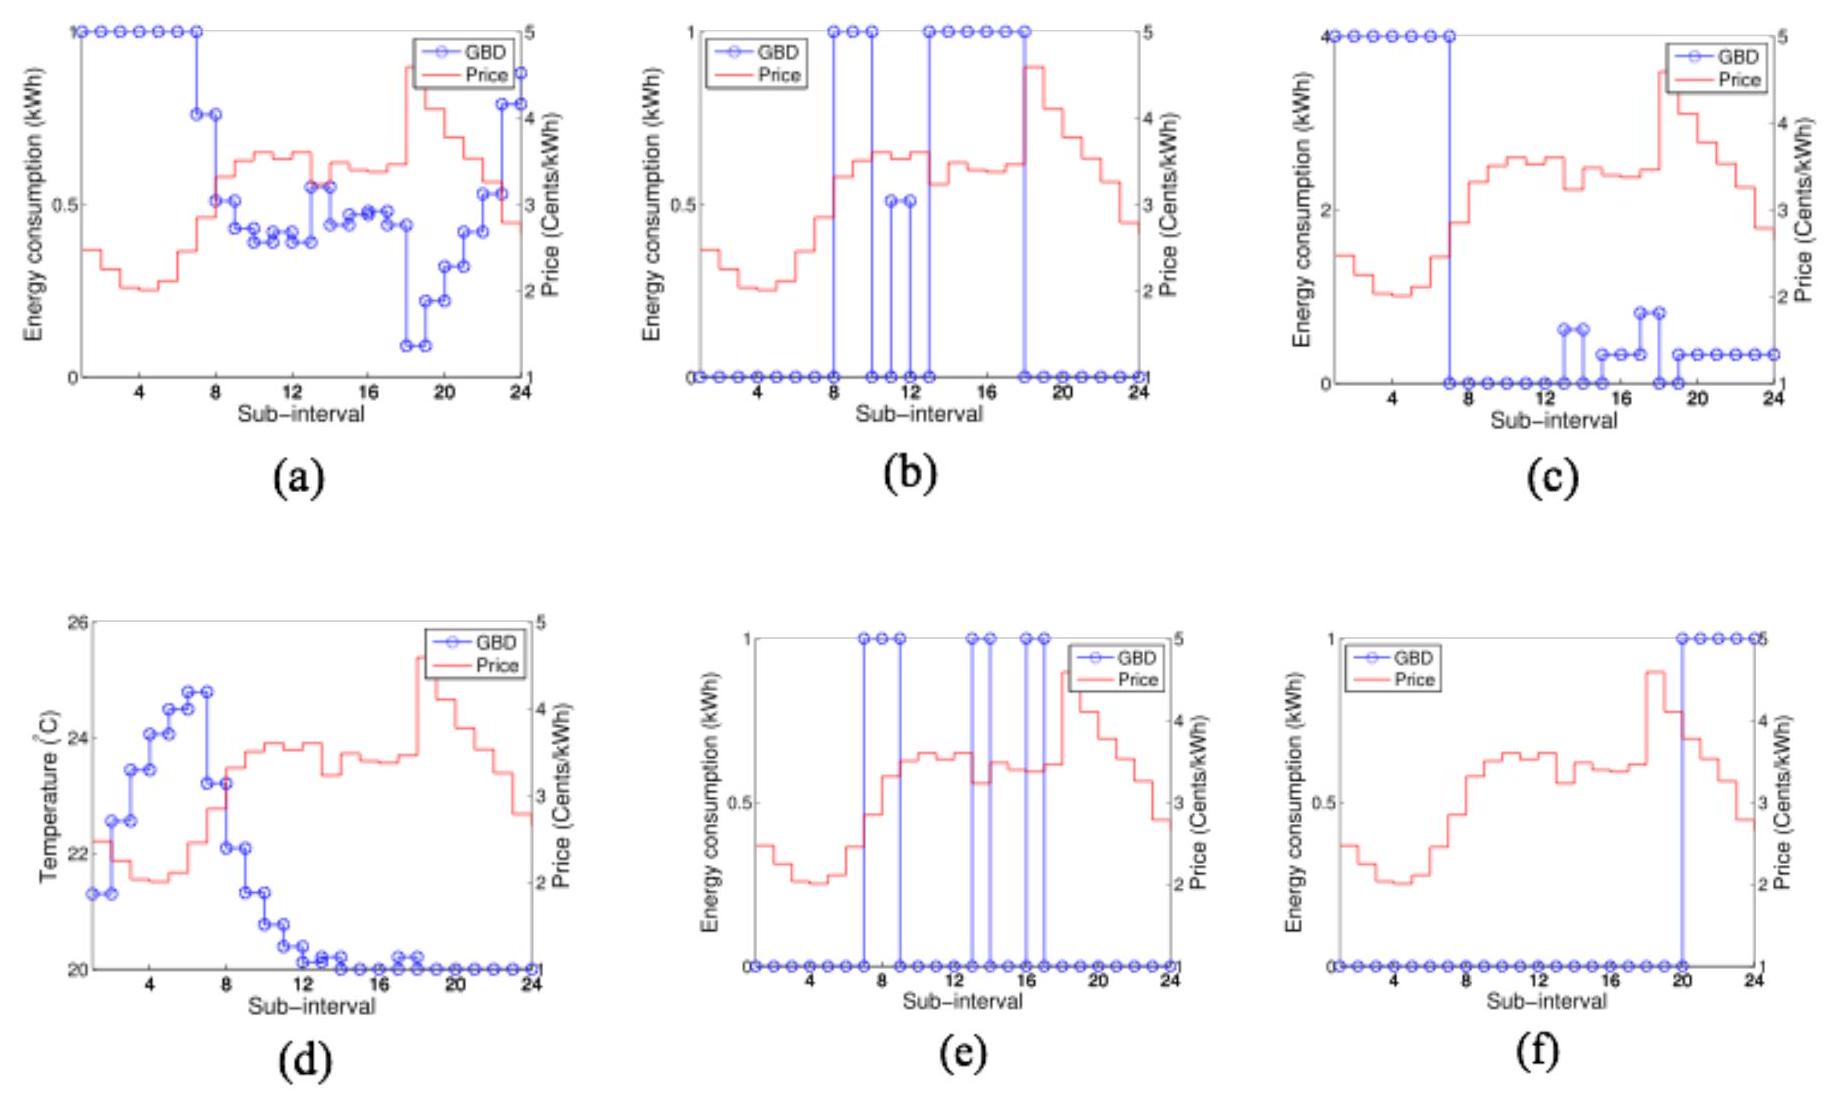
\includegraphics[alt={},max width=\textwidth]{4f5abcf0-f301-43b5-aaf0-9e34a9c79ca8-40_1102_1837_349_630}
\captionsetup{labelformat=empty}
\caption{Fig. 2. ECS of the appliance in each set. Elastic appliance with a (a) memoryless property, (b) full memory property, and (c) partial memory property. (d) Temperature of elastic appliance with a partial memory property. Inelastic appliance with an (e) interruptible operation and (f) uninterruptible operation.}
\end{center}
\end{figure}


\end{document}